
\documentclass[letterpaper,hide notes,xcolor={table,svgnames},pdftex,10pt]{beamer}
\def\showexamples{t}


%\usepackage[svgnames]{xcolor}

%% Demo talk
%\documentclass[letterpaper,notes=show]{beamer}

\usecolortheme{crane}
\setbeamertemplate{navigation symbols}{}

\usetheme{MyPittsburgh}
%\usetheme{Frankfurt}

%\usepackage{tipa}

\usepackage{hyperref}
\usepackage{graphicx,xspace}
\usepackage[normalem]{ulem}

\newcommand\SF[1]{$\bigstar$\footnote{SF: #1}}

\usepackage[default]{sourcesanspro}
\usepackage[T1]{fontenc}

\newcounter{tmpnumSlide}
\newcounter{tmpnumNote}

% old question code
%\newcommand\question[1]{{$\bigstar$ \small \onlySlide{2}{#1}}}
% \newcommand\nquestion[1]{\ifdefined \presentationonly \textcircled{?} \fi \note{\par{\Large \textbf{?}} #1}}
% \newcommand\nanswer[1]{\note{\par{\Large \textbf{A}} #1}}


 \newcommand\mnote[1]{%
   \addtocounter{tmpnumSlide}{1}
   \ifdefined\showcues {~\tiny\fbox{\arabic{tmpnumSlide}}}\fi
   \note{\setlength{\parskip}{1ex}\addtocounter{tmpnumNote}{1}\textbf{\Large \arabic{tmpnumNote}:} {#1\par}}}

\newcommand\mmnote[1]{\note{\setlength{\parskip}{1ex}#1\par}}

%\newcommand\mnote[2][]{\ifdefined\handoutwithnotes {~\tiny\fbox{#1}}\fi
% \note{\setlength{\parskip}{1ex}\textbf{\Large #1:} #2\par}}

%\newcommand\mnote[2][]{{\tiny\fbox{#1}} \note{\setlength{\parskip}{1ex}\textbf{\Large #1:} #2\par}}

\newcommand\mquestion[2]{{~\color{red}\fbox{?}}\note{\setlength{\parskip}{1ex}\par{\Large \textbf{?}} #1} \note{\setlength{\parskip}{1ex}\par{\Large \textbf{A}} #2\par}\ifdefined \presentationonly \pause \fi}

\newcommand\blackboard[1]{%
\ifdefined   \showblackboard
  {#1}
  \else {\begin{center} \fbox{\colorbox{blue!30}{%
         \begin{minipage}{.95\linewidth}%
           \hspace{\stretch{1}} Some space intentionally left blank; done at the blackboard.%
         \end{minipage}}}\end{center}}%
         \fi%
}



%\newcommand\q{\tikz \node[thick,color=black,shape=circle]{?};}
%\newcommand\q{\ifdefined \presentationonly \textcircled{?} \fi}

\usepackage{listings}
\lstset{%
  keywordstyle=\bfseries,
  aboveskip=15pt,
  belowskip=15pt,
  captionpos=b,
  identifierstyle=\ttfamily,
  escapeinside={(*@}{@*)},
  stringstyle=\ttfamiliy,
  frame=lines,
  numbers=left, basicstyle=\scriptsize, numberstyle=\tiny, stepnumber=0, numbersep=2pt}

\usepackage{siunitx}
\newcommand\sius[1]{\num[group-separator = {,}]{#1}\si{\micro\second}}
\newcommand\sims[1]{\num[group-separator = {,}]{#1}\si{\milli\second}}
\newcommand\sins[1]{\num[group-separator = {,}]{#1}\si{\nano\second}}
\sisetup{group-separator = {,}, group-digits = true}

%% -------------------- tikz --------------------
\usepackage{tikz}
\usetikzlibrary{positioning}
\usetikzlibrary{arrows,backgrounds,automata,decorations.shapes,decorations.pathmorphing,decorations.markings,decorations.text}

\tikzstyle{place}=[circle,draw=blue!50,fill=blue!20,thick, inner sep=0pt,minimum size=6mm]
\tikzstyle{transition}=[rectangle,draw=black!50,fill=black!20,thick, inner sep=0pt,minimum size=4mm]

\tikzstyle{block}=[rectangle,draw=black, thick, inner sep=5pt]
\tikzstyle{bullet}=[circle,draw=black, fill=black, thin, inner sep=2pt]

\tikzstyle{pre}=[<-,shorten <=1pt,>=stealth',semithick]
\tikzstyle{post}=[->,shorten >=1pt,>=stealth',semithick]
\tikzstyle{bi}=[<->,shorten >=1pt,shorten <=1pt, >=stealth',semithick]

\tikzstyle{mut}=[-,>=stealth',semithick]

\tikzstyle{treereset}=[dashed,->, shorten >=1pt,>=stealth',thin]

\usepackage{ifmtarg}
\usepackage{xifthen}
\makeatletter
% new counter to now which frame it is within the sequence
\newcounter{multiframecounter}
% initialize buffer for previously used frame title
\gdef\lastframetitle{\textit{undefined}}
% new environment for a multi-frame
\newenvironment{multiframe}[1][]{%
\ifthenelse{\isempty{#1}}{%
% if no frame title was set via optional parameter,
% only increase sequence counter by 1
\addtocounter{multiframecounter}{1}%
}{%
% new frame title has been provided, thus
% reset sequence counter to 1 and buffer frame title for later use
\setcounter{multiframecounter}{1}%
\gdef\lastframetitle{#1}%
}%
% start conventional frame environment and
% automatically set frame title followed by sequence counter
\begin{frame}%
\frametitle{\lastframetitle~{\normalfont(\arabic{multiframecounter})}}%
}{%
\end{frame}%
}
\makeatother

\makeatletter
\newdimen\tu@tmpa%
\newdimen\ydiffl%
\newdimen\xdiffl%
\newcommand\ydiff[2]{%
    \coordinate (tmpnamea) at (#1);%
    \coordinate (tmpnameb) at (#2);%
    \pgfextracty{\tu@tmpa}{\pgfpointanchor{tmpnamea}{center}}%
    \pgfextracty{\ydiffl}{\pgfpointanchor{tmpnameb}{center}}%
    \advance\ydiffl by -\tu@tmpa%
}
\newcommand\xdiff[2]{%
    \coordinate (tmpnamea) at (#1);%
    \coordinate (tmpnameb) at (#2);%
    \pgfextractx{\tu@tmpa}{\pgfpointanchor{tmpnamea}{center}}%
    \pgfextractx{\xdiffl}{\pgfpointanchor{tmpnameb}{center}}%
    \advance\xdiffl by -\tu@tmpa%
}
\makeatother
\newcommand{\copyrightbox}[3][r]{%
\begin{tikzpicture}%
\node[inner sep=0pt,minimum size=2em](ciimage){#2};
\usefont{OT1}{phv}{n}{n}\fontsize{4}{4}\selectfont
\ydiff{ciimage.south}{ciimage.north}
\xdiff{ciimage.west}{ciimage.east}
\ifthenelse{\equal{#1}{r}}{%
\node[inner sep=0pt,right=1ex of ciimage.south east,anchor=north west,rotate=90]%
{\raggedleft\color{black!50}\parbox{\the\ydiffl}{\raggedright{}#3}};%
}{%
\ifthenelse{\equal{#1}{l}}{%
\node[inner sep=0pt,right=1ex of ciimage.south west,anchor=south west,rotate=90]%
{\raggedleft\color{black!50}\parbox{\the\ydiffl}{\raggedright{}#3}};%
}{%
\node[inner sep=0pt,below=1ex of ciimage.south west,anchor=north west]%
{\raggedleft\color{black!50}\parbox{\the\xdiffl}{\raggedright{}#3}};%
}
}
\end{tikzpicture}
}


%% --------------------

%\usepackage[excludeor]{everyhook}
%\PushPreHook{par}{\setbox0=\lastbox\llap{MUH}}\box0}

%\vspace*{\stretch{1}

%\setbox0=\lastbox \llap{\textbullet\enskip}\box0}

\setlength{\parskip}{\fill}

\newcommand\noskips{\setlength{\parskip}{1ex}}
\newcommand\doskips{\setlength{\parskip}{\fill}}

\newcommand\xx{\par\vspace*{\stretch{1}}\par}
\newcommand\xxs{\par\vspace*{2ex}\par}
\newcommand\tuple[1]{\langle #1 \rangle}
\newcommand\code[1]{{\sf \footnotesize #1}}
\newcommand\ex[1]{\uline{Example:} \ifdefined \presentationonly \pause \fi
  \ifdefined\showexamples#1\xspace\else{\uline{\hspace*{2cm}}}\fi}

\newcommand\ceil[1]{\lceil #1 \rceil}


\AtBeginSection[]
{
   \begin{frame}
       \frametitle{Outline}
       \tableofcontents[currentsection]
   \end{frame}
}



\pgfdeclarelayer{edgelayer}
\pgfdeclarelayer{nodelayer}
\pgfsetlayers{edgelayer,nodelayer,main}

\tikzstyle{none}=[inner sep=0pt]
\tikzstyle{rn}=[circle,fill=Red,draw=Black,line width=0.8 pt]
\tikzstyle{gn}=[circle,fill=Lime,draw=Black,line width=0.8 pt]
\tikzstyle{yn}=[circle,fill=Yellow,draw=Black,line width=0.8 pt]
\tikzstyle{empty}=[circle,fill=White,draw=Black]
\tikzstyle{bw} = [rectangle, draw, fill=blue!20, 
    text width=4em, text centered, rounded corners, minimum height=2em]
    
    \newcommand{\CcNote}[1]{% longname
	This work is licensed under the \textit{Creative Commons #1 3.0 License}.%
}
\newcommand{\CcImageBy}[1]{%
	\includegraphics[scale=#1]{creative_commons/cc_by_30.pdf}%
}
\newcommand{\CcImageSa}[1]{%
	\includegraphics[scale=#1]{creative_commons/cc_sa_30.pdf}%
}
\newcommand{\CcImageNc}[1]{%
	\includegraphics[scale=#1]{creative_commons/cc_nc_30.pdf}%
}
\newcommand{\CcGroupBySa}[2]{% zoom, gap
	\CcImageBy{#1}\hspace*{#2}\CcImageNc{#1}\hspace*{#2}\CcImageSa{#1}%
}
\newcommand{\CcLongnameByNcSa}{Attribution-NonCommercial-ShareAlike}

\newenvironment{changemargin}[1]{% 
  \begin{list}{}{% 
    \setlength{\topsep}{0pt}% 
    \setlength{\leftmargin}{#1}% 
    \setlength{\rightmargin}{1em}
    \setlength{\listparindent}{\parindent}% 
    \setlength{\itemindent}{\parindent}% 
    \setlength{\parsep}{\parskip}% 
  }% 
  \item[]}{\end{list}} 




\title{Lecture 18 --- Concurrency \& Synchronization in POSIX }

\author{Jeff Zarnett \\ \small \texttt{jzarnett@uwaterloo.ca}}
\institute{Department of Electrical and Computer Engineering \\
  University of Waterloo}
\date{\today}


\begin{document}

\begin{frame}
  \titlepage

 \end{frame}


\begin{frame}
\frametitle{Concurrency with pthreads}

Earlier we saw pthreads \& how we can use them: multithreaded programs. 

There are, accordingly, pthread routines for working with mutual exclusion.

\end{frame}


\begin{frame}
\frametitle{Mutexes and pthreads}

\texttt{pthread\_mutex\_init}: used to create a new mutex variable and returns it, with type \texttt{pthread\_mutex\_t}. 

It takes an optional parameter, the attributes (the details of which are not important at the moment, but relate mostly to priorities).

We can initialize it using null, or:

\texttt{pthread\_mutex\_t mymutex = PTHREAD\_MUTEX\_INITIALIZER;} 

\end{frame}

\begin{frame}
\frametitle{Mutexes and pthreads}

When created, by default, the mutex is unlocked. 

There are three methods related to using the mutex; two to lock it and one to unlock it, all of which take as a parameter the mutex to (un)lock. 

The unlock method, \texttt{pthread\_mutex\_unlock} is self-explanatory. 

The two kinds of lock are \texttt{pthread\_mutex\_lock}, which is blocking, and \texttt{pthread\_mutex\_trylock}, which is nonblocking. 

Attempting to unlock a mutex that is not currently locked is an error.

Also an error if one thread attempts to unlock a mutex owned by another.

\end{frame}

\begin{frame}
\frametitle{Destroying the Mutex}

To destroy a mutex, there is a method \texttt{pthread\_mutex\_destroy}. 

It cleans up a mutex and should be used when finished with it.

If attributes were created with \texttt{pthread\_mutexattr\_init} they should be destroyed with \texttt{pthread\_mutexattr\_destroy}.

\end{frame}

\begin{frame}
\frametitle{Destruction Aborted}

An attempt to destroy the mutex may fail if the mutex is currently locked. 

The specification says that destroying an unlocked mutex is okay, but attempting to destroy a locked one results in undefined behaviour. 

Undefined behaviour is, in the words of the internet, the worst thing ever.

It means code might work some of the time or on some systems, but not others. 

Or it could work fine for a while and then break suddenly later.
\end{frame}

\begin{frame}
\frametitle{Condition Variables}

Condition variables are another way to achieve synchronization.

A condition variable allows synchronization based on the value of the data. 

Instead of locking a mutex, checking a variable, and then unlocking the mutex, we could achieve the same goal without constantly polling. 

We can think of condition variables as ``events'' that occur.

\end{frame}

\begin{frame}
\frametitle{Condition Variables: Events}

An event is similar to, but slightly different from, a counting semaphore. 

When an event occurs we can:\\
\quad Signal either one thread waiting for that event to occur, or\\
\quad Broadcast (signal) to all threads waiting for the event. 

If a thread signals a condition variable that an event has occurred, but no thread is waiting for that event, the event is ``lost''. 

\end{frame}

\begin{frame}
\frametitle{Condition Variables and pthreads}

To create a \texttt{pthread\_cond\_t} (condition variable type), the function is \texttt{pthread\_cond\_init}.

To destroy them, \texttt{pthread\_cond\_destroy}. 

As before, we can initialize them with attributes, and there are functions to create and destroy the attribute structures, too. 

\end{frame}

\begin{frame}
\frametitle{Condition Variables as a Building Block}

Condition variables are a building block and must be paired with a mutex. 

To wait on a condition variable, the function \texttt{pthread\_cond\_wait} takes two parameters: the condition variable and the mutex. 

This routine should be called only while the mutex is locked.

\end{frame}

\begin{frame}
\frametitle{Condition Variables as a Building Block}

It will automatically release the mutex while it waits for the condition. 

When the condition is true then the mutex will be automatically locked again so the thread may proceed. 

The programmer then unlocks the mutex when the thread is finished with it. 

\end{frame}

\begin{frame}
\frametitle{Condition Variables}

There is \texttt{pthread\_cond\_signal} that signals a provided condition variable. 

There is also \texttt{pthread\_cond\_broadcast} that signals all threads waiting. 

It is (almost always) a logical error to signal or broadcast on a condition variable before some thread is waiting on it.

\end{frame}

\begin{frame}
\frametitle{Condition Variable Example}

[This code is too big for slides; see notes.]

\end{frame}

\begin{frame}
\frametitle{Monitors}

A condition variable can be used to create a \alert{monitor}.

Analogy: in object-oriented programming we package up data and functions inside a class to make errors less likely and to improve the design. 

When we use a monitor we are packaging up the shared data and operations on that data to avoid problems of synchronization and concurrency.

\end{frame}

\begin{frame}
\frametitle{Monitors}

Goal: make it so that programmers do not need to code the synchronization part directly, making it less likely a programmer makes an error.

\begin{center}
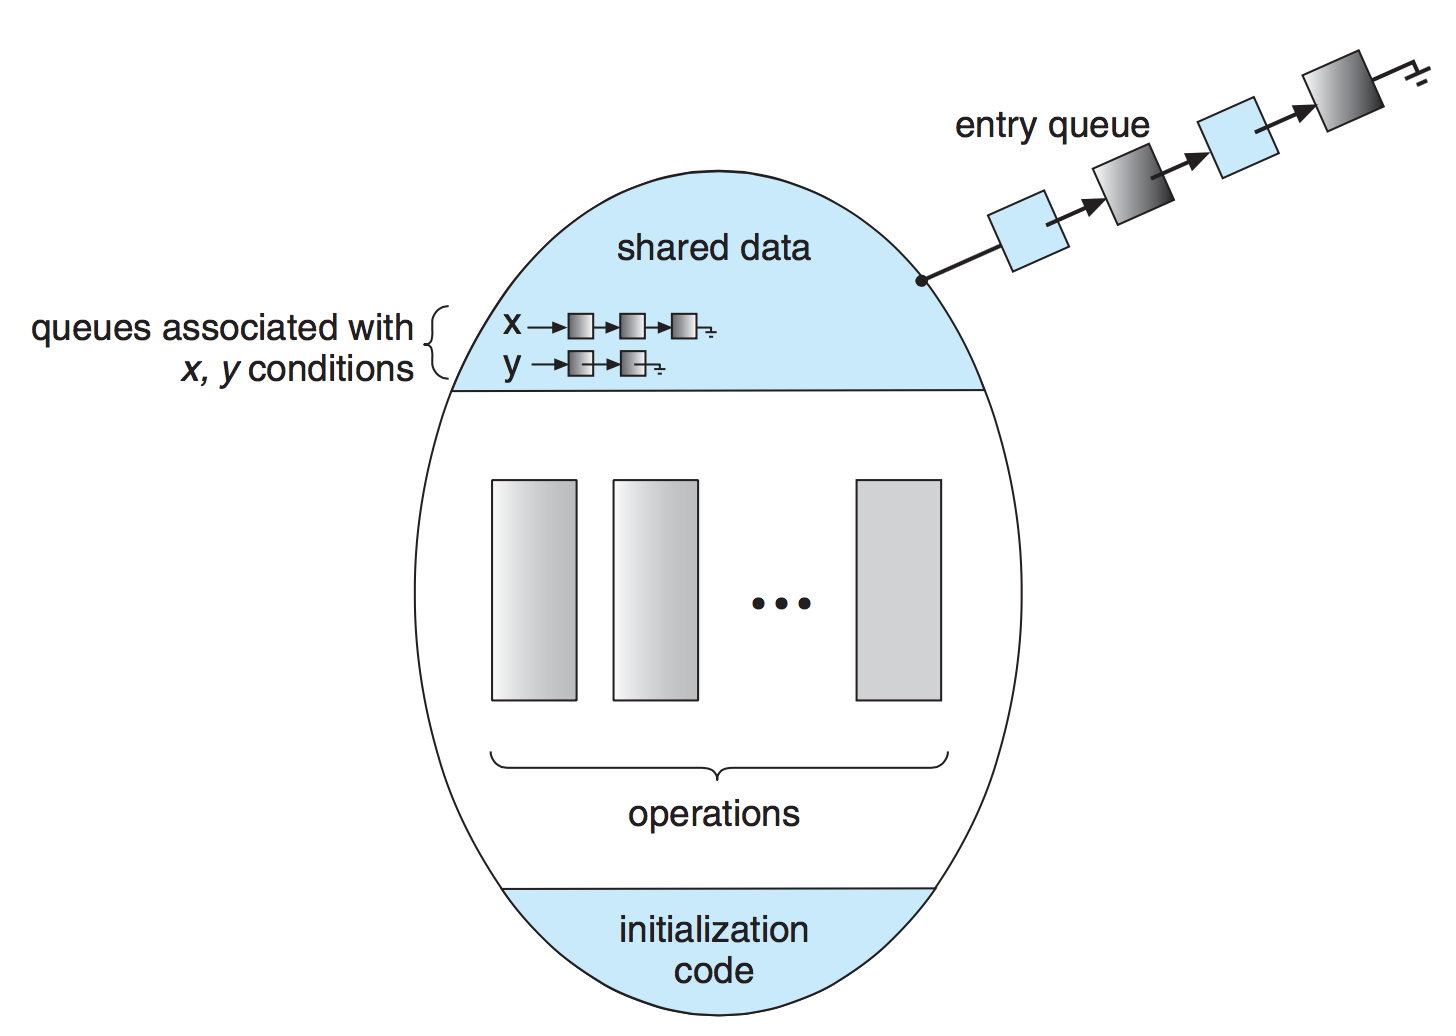
\includegraphics[width=0.65\textwidth]{images/sync-monitor.png}
\end{center}

\end{frame}

\begin{frame}
\frametitle{Monitor Example}


Suppose there are processes $P$ and $Q$ and a condition variable $x$. 

If $P$ signals on $x$ when $Q$ is waiting, there are two things we can do:\\
\quad \alert{signal-and-wait} or \alert{signal-and-continue}. 

Signal-and-continue seems logical, in one sense: $P$ is already running, so why do the extra work to switch? 

On the other hand, by the time $P$ exits the monitor on its own, the condition $Q$ was waiting for might no longer be true.

Some programming languages opt for a compromise: after signalling, $P$ must immediately leave the monitor.

\end{frame}

\begin{frame}
\frametitle{Monitors and \texttt{synchronized}}

The idea of monitors should be familiar to you if you have used the Java \texttt{synchronized} keyword. 

In Java we can declare a method to be \texttt{synchronized}.\\
\quad Then there is a lock created around that method. 

Only one thread can be inside that method at a time.

If a second would like to call that method on the same instance, it will be placed in the entry set for the lock.

\end{frame}

\begin{frame}[fragile]
\frametitle{Java Synchronization}


In Java we can make a method \texttt{synchronized} or define a block as synchronized:

\begin{verbatim}
public synchronized void doSomething() {
    // Synchronized area
}
\end{verbatim}



\begin{verbatim}
public void exampleMethod() {
    synchronized( object ) { // Lock must be acquired to enter
           // Critical section 
    } // Lock is automatically released.
}
\end{verbatim}


\end{frame}

\begin{frame}
\frametitle{UNIX Concurrency Mechanisms}

UNIX also has semaphores (not just in the pthreads). 

The semaphore in UNIX is general, and maintains a few pieces of extra data:

\begin{itemize}
    \item The value of the semaphore.
    \item Process ID of the last process to operate it.
    \item Number of processes waiting on a value greater than the current value.
    \item Number of processes waiting for the value to be 0.
\end{itemize}

\end{frame}

\begin{frame}
\frametitle{UNIX Semaphores}

UNIX semaphores are technically created in sets of one or more. 

It is possible to manage semaphores en masse with a system call (\texttt{semctl}).

This then performs the requested operation on all of the semaphores in the set. 

There is also a \texttt{sem\_op} system call that takes as an argument, a list of semaphore operations, each defined on one of the semaphores in the set. 

When \texttt{sem\_op} is used, the indicated operations are performed one at a time.

\end{frame}

\begin{frame}
\frametitle{UNIX \texttt{sem\_op}}

The meanings of \texttt{sem\_op} can be:
\begin{itemize}
    \item \texttt{sem\_op} positive
    \item \texttt{sem\_op} 0
    \item \texttt{sem\_op} negative and its absolute value $\leq$ to the semaphore value
    \item \texttt{sem\_op} negative and its absolute value $>$ the semaphore value
\end{itemize}

\end{frame}

\begin{frame}
\frametitle{Linux Kernel Concurrency Mechanisms}

The Linux kernel provides operations that are guaranteed to execute atomically, to avoid simple race conditions.

Uniprocessor system: CPU can't be interrupted until the operation is finished.

Multiprocessor system: the variable is locked until the operation is finished.

\end{frame}

\begin{frame}
\frametitle{Linux Kernel Concurrency Mechanisms}

There are two types of atomic operations:\\
\quad Those that operate on integers; and\\
\quad Those that operate on a single bit in a bitmap. 

On some architectures, the atomic operations are translated into uninterruptible assembly instructions.

On others, the memory bus is locked to ensure the operation is atomic.

\end{frame}


\begin{frame}
\frametitle{Linux Kernel Concurrency Mechanisms}

Rather than just using an integer for atomic integer operations, there is a defined type \texttt{atomic\_t}. 

This ensures that only atomic operations can be used on this data type and that atomic operations can only be used on that data type. 

This prevents programming errors and hides architecture-specific implementation details.


\end{frame}

\begin{frame}
\frametitle{Linux Atomic Operations}

{\scriptsize
\begin{center}
\begin{tabular}{l|l}
	\textbf{Function} & \textbf{Description}\\\hline

	\texttt{ATOMIC\_INIT( int i )} & At declaration, initialize an \texttt{atomic\_t} to \texttt{i}\\\hline

\texttt{int atomic\_read( atomic\_t *v )} &  Read the integer value of \texttt{v}\\\hline

\texttt{void atomic\_set( atomic\_t *v, int i )} & Set \texttt{v} equal to \texttt{i}\\\hline

\texttt{void atomic\_add( int i, atomic\_t *v )} & Add \texttt{i} to \texttt{v}\\\hline

\texttt{void atomic\_sub( int i, atomic\_t *v )} & Subtract \texttt{i} from \texttt{v}\\\hline

\texttt{void atomic\_inc( atomic\_t *v )} & Add 1 to \texttt{v}\\\hline

\texttt{void atomic\_dec( atomic\_t *v )} & Subtract 1 from \texttt{v}\\\hline

\texttt{int atomic\_sub\_and\_test( int i, atomic\_t *v )} & Subtract \texttt{i} from \texttt{v}; return true if 0; otherwise false\\\hline

\texttt{int atomic\_add\_negative( int i, atomic\_t *v )} & Add \texttt{i} to \texttt{v}; return true if negative; otherwise false\\\hline

\texttt{int atomic\_dec\_and\_test( atomic\_t *v )} & Decrement \texttt{v} by 1; return true if 0; otherwise false\\\hline

\texttt{int atomic\_inc\_and\_test( atomic\_t *v )} & Increment \texttt{v} by 1; return true if 0; otherwise false\\ \hline\hline

\texttt{void set\_bit( int n, void *addr )} &  Set the $n^{th}$ bit starting from \texttt{addr}\\\hline

\texttt{void clear\_bit( int n, void *addr )} &  Clear the $n^{th}$ bit starting from \texttt{addr}\\\hline

\texttt{void change\_bit( int n, void *addr )} &  Flip the value of the $n^{th}$ bit starting from \texttt{addr}\\\hline

\texttt{int test\_and\_set\_bit( int n, void *addr )} &  Set $n^{th}$ bit starting from \texttt{addr}; return previous value\\\hline

\texttt{int test\_and\_clear\_bit( int n, void *addr )} &  Clear $n^{th}$ bit starting from \texttt{addr}; return previous value\\\hline

\texttt{int test\_and\_change\_bit( int n, void *addr )} &  Flip $n^{th}$ bit starting from \texttt{addr}; return previous value\\\hline

\texttt{int test\_bit( int n, void *addr )} &  Return value of $n^{th}$ bit starting from \texttt{addr}\\\hline

\end{tabular}
\end{center}
}

\end{frame}

\begin{frame}
\frametitle{Linux Spinlocks}

Another technique for protecting a critical section in Linux is the \alert{spinlock}. 

This is a handy way to implement constant checking to acquire a lock.

Unlike semaphores where the process is blocked if it fails to acquire the lock, a thread will constantly try to acquire the lock. 

The implementation is an integer that is checked by a thread.

\end{frame}

\begin{frame}[fragile]
\frametitle{Linux Spinlocks}

This is very inefficient; it would be better to let another thread execute.

Except where the amount of time waiting on the lock is less than it would take to block the process, switch to another, and unblock it when the value changes.

\begin{verbatim}
spin_lock( &lock )
    /* Critical Section */
spin_unlock( & lock )
\end{verbatim}

\end{frame}

\begin{frame}
\frametitle{Linux Reader-Writer Spinlock}

There are \alert{reader-writer-spinlocks}. 

Allow multiple readers but give exclusive access to a writer. 

This is implemented as a 24-bit reader counter and an unlock flag:
\begin{center}
\begin{tabular}{l|l|l}
	\textbf{Counter} & \textbf{Flag} & \textbf{Interpretation}\\\hline
	0 & 1 & The spinlock is released and available. \\
	0 & 0 & The spinlock has been acquired for writing.\\
	$n$ ($n > 0$) & 0 & The spin lock has been acquired for reading by $n$ threads.\\
	$n$ ($n > 0$) & 1 & Invalid state.\\
\end{tabular}
\end{center}

\end{frame}

\end{document}

